\documentclass[czech, kiv, ba, he, iso690alph, pdf]{fasthesis}

\usepackage{url}
\usepackage{float}

\title{Implementace modulu pro import údajů RÚIAN}
\author{Martin}{Schön}{}{}
\supervisor{Martin Bíkl, Ing. Petr Přibyl, Ing. Martin Zíma Ph.D.}
\stagworkid{100718}
\assignment{figures/zadani.pdf}
\signdate{31}{12}{2024}{V Plzni}
\addbibresource{bib.bib}
\abstract{Text abstraktu v~jazyce práce, tj. zde česky.}
{The abstract text in a secondary language, here in English.}
\keywords{}
\acknowledgement{Text poděkování.}

\begin{document}
\frontpages[tm]
\tableofcontents
%---------------------------------------------------------------------------
\chapter{Úvod}
%TODO: Úvod

\chapter{RÚIAN}
\section{Co je to RÚIAN}
RÚIAN je zkratka pro Registr územní identifikace, adres a nemovitostí. 
Jedná se o státní informační systém v České republice, který obsahuje informace o adresách, budovách, parcelách a dalších objektech. 
Systém je spravován Českým úřadem zeměměřickým a katastrálním (ČÚZK). 
Data jsou využívána v mnoha oblastech. 
Jednotlivé prvky jsou zobrazovány na mapách státního mapového díla a digitální mapě veřejné správy.

\section{Získaní dat}
Data z RÚIAN jsou veřejně dostupná a lze je získat z webové služby na adrese \url{https://vdp.cuzk.cz/vdp/ruian}.
V této aplikaci je možné vyhledávat konkrétní prvky nebo ověřit jejich existenci.
Cílem této práce je výměnný formát z této služby odkud je třeba stáhnout, zpracovat a uložit do databáze.

\section{VFR -- Výměnný formát RÚIAN}
Výměnný formát RÚIAN je služba poskytující data.
Je možné stahovat data dle zadaných formátů: Standardní, Historický a Speciální.
Každý formát obsahuje dodatečně parametry, které je možné nastavit.
Data z VFR jsou ve formátu XML.
Každý element obsahuje atributy, které obsahují informace o dané entitě (Tabulce).
\pagebreak
\begin {itemize}
    \item \textbf{Standardní} -- obsahuje úplná nebo přírůstková data.
    \begin {itemize}
        \item Časový rozsah: Přírůstky od data / Úplná kopie
        \item Územní prvky: Stát až ZJS / Obec a podřadné
        \item Datová sada: Základní / Kompletní
        \item Výběr z údajů: Základní údaje / Gen. hranice, Originální hranice, Vlajky a znaky
        \item Územní omezení: ČR / Kraj (VÚSC) / ORP / Obec
    \end {itemize}
    \item \textbf{Historický} -- obsahuje historická data.
    \begin {itemize}
        \item Časový rozsah: Přírůstky od data / Úplná kopie
        \item Územní prvky: Stát až ZJS / Obec a podřadné
        \item Územní omezení: ČR / Kraj (VÚSC) / ORP / Obec
    \end {itemize}
    \item \textbf{Speciální} -- obsahuje speciální data.
    \begin {itemize}
        \item Časový rozsah: Přírůstky od data / Úplná kopie
        \item Výběr z údajů: Číselníky / Vazby / Vazby a číselníky
        \item Kategorie: Všechny / Geodetické body / Nerostné bohatství
    \end {itemize}
\end {itemize}

\section{Tabulky}
Data z RÚIAN jsou rozdělena do několika tabulek.
Jak je vidět na obrázku \ref{fig:ruian_tables}, každá tabulka obsahuje jiné informace.
Některé tabulky obsažené v RÚIAN jsou nepotřebné. 
Příkladem může být tabulka \textit{Stát}, která obsahuje informace o státu Česká republika.
Ovšem RÚIAN obsahuje pouze informace o České republice, tudíž tato tabulka je nadbytečná.
Definice, které tabulky budou zpracovány a které budou ignorovány, záleží na specifikaci v XSD (XML Schema Definition) souborech v dokumentaci VFR. 

\pagebreak
\begin{figure}[H]
    \centering
    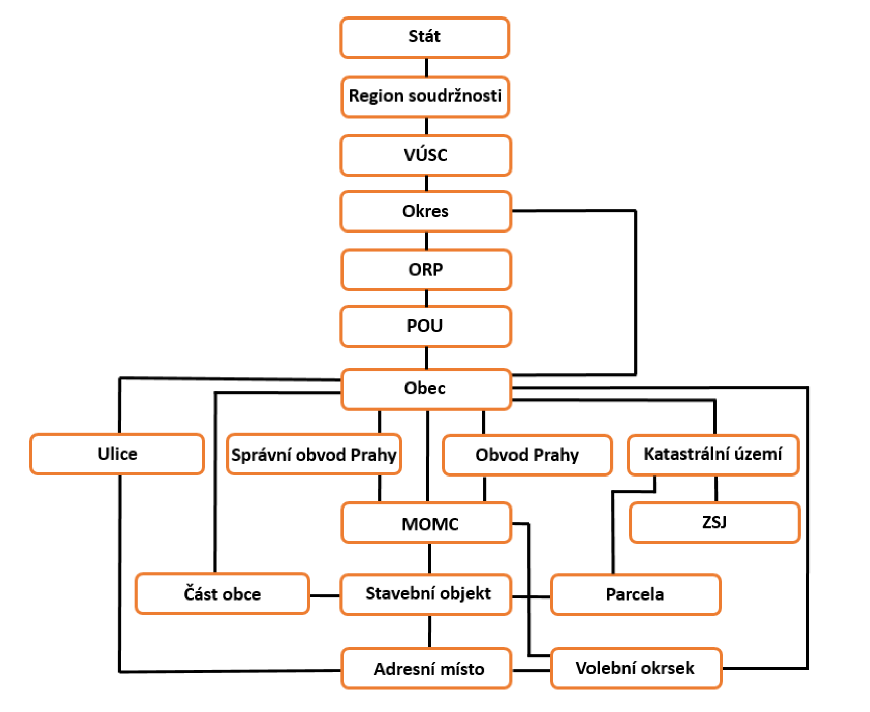
\includegraphics[width=\textwidth]{figures/ruian_tables.png}
    \caption{Tabulky RÚIAN}
    \label{fig:ruian_tables}
\end{figure}

\section{Uložení dat}
Vzhledem k formátu dat z VFR, je potřeba vybrat vhodný způsob uložení dat.
Jednou z možností je uložení dat do relační databáze.
Elementy XML souboru budou mapovány na tabulky v databázi.
Další možností je uložení dat do NoSQL databáze.
Vzhledem k tomu, že data z VFR mají pevnou strukturu, je vhodnější uložení do relační databáze s využitím SQL jazyka.

\chapter{Databáze}
\section{Microsoft SQL}
\section{PostgreSQL}
\section{Oracle}
\section{Komunikace s databází}
\section{Mapování dat / ORM}

\chapter{Konfigurační soubor}
\section{Formát}
\section{Nastavení}

\chapter{Technologie}
\section{Rest API}
\section{Spring Framework}
\section{Docker}




%---------------------------------------------------------------------------
\appendix
\chapter{První příloha}
\backmatter
\printbibliography
\setbackpageqrcode
\backpage
\end{document}